\documentclass[conference]{IEEEtran}
\IEEEoverridecommandlockouts

\usepackage{cite}
\usepackage{amsmath,amssymb,amsfonts}
\usepackage{graphicx}
\usepackage{textcomp}
\usepackage{xcolor}
\usepackage{booktabs}
\usepackage{url}

\def\BibTeX{{\rm B\kern-.05em{\sc i\kern-.025em b}\kern-.08em
    T\kern-.1667em\lower.7ex\hbox{E}\kern-.125emX}}

\begin{document}

\title{Conversation-Context Conditioned Naturalness Distributions for Speech-to-Speech Evaluation\\
\thanks{Full funding acknowledgments will be added after acceptance.}
}

\author{Anonymized submission to IEEE SLT 2026}
% \author{\IEEEauthorblockN{Ashish Hallur\IEEEauthorrefmark{1}, Sathvik Manikantan Napa Ugandhar\IEEEauthorrefmark{1}, Thomas Thebaud\IEEEauthorrefmark{1}, \\
% Georgi Tinchev\IEEEauthorrefmark{2}, Venkatesh Ravichandran\IEEEauthorrefmark{2}, Laureano Moro-Velazquez\IEEEauthorrefmark{1}}
% \IEEEauthorblockA{\IEEEauthorrefmark{1}\textit{Department of Electrical and Computer Engineering, Johns Hopkins University}, Baltimore, MD, USA\\
% Email: ahallur1@jhu.edu}
% \IEEEauthorblockA{\IEEEauthorrefmark{2}\textit{Amazon AGI}, Seattle, WA, USA}}

\maketitle

\begin{abstract}
Speech-to-speech (S2S) systems can produce fluent spoken responses, but fluency alone does not guarantee conversational naturalness.
A response may be intelligible and semantically appropriate while sounding atypical in duration, rhythm, pausing, pitch variation, or affect for the conversation that preceded it.
We present a conversation-context conditioned evaluator that learns distributions over response-side speech measurements from natural dyadic interaction.
Each example is an adjacent-turn pair: a preceding turn from one speaker is used as context, and the next cross-speaker turn supplies the response measurements to be modeled.
Building on DISTRIB's reference-based prosody and rhythm checks, we replace static matched ranges with learned conditional distributions over 12 naturalness-relevant response metrics.
We train history-aware CVAE models on 85,566 natural Seamless Interaction examples and test on 1,146 held-out natural examples, while using a TRACE-derived EmotiVoice set as an external unnatural probe.
Across 16 history and embedding conditions, the best natural-response predictor uses only interpretable metric and context features with a five-turn history (MSE 0.0250, $R^2=0.9748$).
The strongest natural-vs-EmotiVoice separation is obtained with VoxProfile/Whisper embeddings and a seven-turn history ($\Delta$LL 1.556), while three embedding-aware conditions form the top balanced tier.
A 10-listener study further confirms that TRACE-derived EmotiVoice clips are perceived as less natural than natural/reference clips (2.73 vs. 4.49 MOS), supporting their use as an external unnaturalness probe.
\end{abstract}

\begin{IEEEkeywords}
speech-to-speech evaluation, conversational naturalness, prosody, rhythm, conditional generative modeling, speech embeddings
\end{IEEEkeywords}

\section{Introduction}
Spoken conversation is organized through more than lexical content.
Speakers coordinate turns using timing, prosody, pause structure, and affective stance, and these cues help make an exchange sound smooth rather than merely intelligible \cite{riest_anticipation_2015, levinson_turn-taking_2016, koiso_analysis_1998}.
S2S systems are increasingly able to generate fluent speech, but generated turns can still violate the behavioral ranges that are typical for a given conversational context.
For example, a response may begin after an unusual delay, compress pitch variation in an expressive exchange, speak at an implausible rate, or use affective cues that do not match the preceding turn.
Text-based metrics, task success, and global listener ratings remain useful, but they often do not identify which speech-native dimensions make an output sound unnatural \cite{omahony_combining_2022}.

DISTRIB introduced a reference-based evaluation view: extract prosodic and rhythmic measurements from an S2S output, compare them with matched human conversational regimes, and report interpretable deviations rather than a single opaque score \cite{DISTRIB}.
That approach is intentionally simple, but it treats reference regimes as static tables.
The present paper asks a complementary question: can we learn a conditional distribution over response behavior from the immediately preceding turn and recent dialogue history?
Instead of asking whether an output falls inside a broad matched percentile range, we ask whether its response measurements are likely under a distribution expected for this particular conversational context.

We use the term \emph{conditioning turn} for the preceding speaker turn and \emph{response turn} for the next cross-speaker turn.
Together they form an \emph{adjacent-turn pair}.
The conditioning turn is not an LLM instruction or text prompt; it is the actual speech segment that came immediately before the response in a dyadic conversation.
For each pair, we extract interpretable speech measurements from both sides, optionally add learned speech embeddings from the conditioning turn, and model the response-side measurements.
The core object is
\begin{equation}
    p_{\theta}(y_t \mid x_t, h_t^{(H)}),
    \label{eq:conditional_distribution}
\end{equation}
where $x_t$ describes the current conditioning turn, $h_t^{(H)}$ contains up to $H$ preceding turns from the same interaction, and $y_t$ is a vector of response-side naturalness measurements.

This paper makes five contributions.
First, we convert Seamless Interaction conversations into adjacent-turn examples for distributional S2S evaluation.
Second, we define a 12-metric response target space covering duration, lexical length, pitch variation, voicing, rate, pausing, and dimensional affect.
Third, we compare interpretable-only and embedding-augmented history-aware CVAE models over history windows $H\in\{1,3,5,7\}$.
Fourth, we evaluate each model on two axes: prediction of held-out natural responses and likelihood separation between natural responses and a TRACE-derived EmotiVoice probe \cite{TRACE}.
Fifth, we report listener ratings showing that the TRACE-derived EmotiVoice condition is perceptually less natural than natural/reference speech.

\section{Related Work}
\subsection{Speech-Native S2S Evaluation}
S2S evaluation has inherited many tools from automatic speech recognition, text generation, and text-to-speech evaluation.
These methods measure important aspects of output quality, but they can miss conversational timing, turn-taking fit, prosodic expressivity, and context-appropriate speaking behavior.
Subjective ratings are essential, yet they are expensive and often provide limited diagnostic detail.
Recent studies of spoken dialogue systems show that speech rate, prosody, and interaction partner behavior shape user experience and conversational dynamics, reinforcing the need for evaluation signals that remain in the speech domain \cite{dowding_user_2024, xie_speaking_2024, jung_comparison_2025}.
Our goal is not to replace human evaluation, but to provide a scalable diagnostic that identifies which measurable dimensions of a response deviate from natural conversational behavior.

\subsection{Conversational Prosody and Timing}
Conversational speech differs from read speech in prosodic and temporal structure \cite{howell1991comparison, hazan2010does}.
Prosodic variation, especially fundamental-frequency ($F_0$) range and variability, is associated with emotion, communicative intent, prominence, and discourse structure \cite{banziger_role_2005, pell_emotional_2011, xu_speech_2005, sluijter_acoustic_1996, sluijter_spectral_1996}.
Temporal organization also matters: speaking rate, articulation rate, and pausing shape perceived tempo and turn-taking behavior \cite{tauroza_speech_1990, goldman1958speech, campione2002large, pellegrino_automatic_2004, jiao_estimating_2015, morgan_combining_1998}.
Because these behaviors vary with interactional state, a naturalness evaluator should compare a response with expectations for its local conversation, not with a single global baseline \cite{fusaroli_dialog_2014, wynn_conversational_2024}.

\subsection{Distributional Modeling and Speech Embeddings}
A single preceding turn can allow many natural responses.
A useful evaluator should therefore represent a distribution over plausible response behaviors rather than only a point prediction.
Conditional variational autoencoders (CVAEs) provide a standard way to model output variability under observed context using a latent variable \cite{kingma2013vae, sohn2015cvae}.
Interpretable speech metrics offer transparency, but they may not capture all acoustic or paralinguistic information available in the conditioning turn.
We therefore compare models that use only interpretable metric and context features with models that also use two learned speech representations: 1,024-dimensional Trillsson embeddings for non-semantic speech information \cite{shor2022trillsson}, and a 1,280-dimensional VoxProfile/Whisper stream derived from Whisper representations \cite{radford2023whisper, feng2025vox}.

\section{Data and Measurements}
\subsection{Terms Used in This Paper}
Table~\ref{tab:terminology} defines the main study-specific terms.
The table is included because several terms have overloaded meanings outside this work.

\begin{table}[t]
\centering
\caption{Reader-facing terminology used throughout the paper.}
\label{tab:terminology}
\scriptsize
\setlength{\tabcolsep}{3.2pt}
\begin{tabular}{p{0.31\columnwidth}p{0.61\columnwidth}}
\toprule
Term & Meaning in this paper \\
\midrule
Adjacent-turn pair & Two neighboring cross-speaker turns: a conditioning turn followed by the response turn being modeled. \\
Conditioning turn & The preceding speech segment used as context for evaluation; not an LLM instruction. \\
History window $H$ & The number of earlier turns from the same interaction made available to the model. \\
Interpretable features & Measured speech, timing, affect, and interaction-context variables with direct diagnostic meaning. \\
Embedding-augmented condition & A model that adds Trillsson, VoxProfile/Whisper, or both embedding streams to the interpretable features. \\
TRACE-derived probe & EmotiVoice-based synthetic or voice-converted dyadic clips from TRACE, reused here as an external unnaturalness stress test. \\
\bottomrule
\end{tabular}
\end{table}

\subsection{Natural Adjacent-Turn Examples}
We construct natural examples from Seamless Interaction, a large dyadic English conversation corpus containing naturalistic and improvised face-to-face interactions \cite{seamless_interaction}.
Word-level transcript events from the same speaker are merged when separated by at most 1.0 s, and VAD regions are merged with the same threshold.
Transcript boundaries are refined against overlapping VAD regions or VAD regions within a 0.5 s tolerance.
We retain adjacent turns only when the speaker changes, remove short backchannel-only turns, and keep conditioning and response segments between 3 and 15 s.
Pairs with more than 0.25 s of overlap or more than 1.0 s of response latency are excluded.

The refined experiments use the source dataset partitions directly: Seamless train/dev examples are used for training, and Seamless test examples are held out for natural-response evaluation.
After filtering and embedding alignment, the reported experiments contain 85,566 natural training examples and 1,146 held-out natural examples.

\subsection{TRACE-Derived EmotiVoice Probe}
To test whether models trained on natural responses assign lower likelihood to unnatural speech, we use the EmotiVoice-derived conditions from TRACE as an external probe \cite{TRACE}.
TRACE constructs synthetic and voice-converted dyadic clips that are intended to disrupt natural conversational entrainment.
Here, we do not treat TRACE as a general benchmark dataset; we use its corresponding row directories as a deliberately unnatural stress test.
The same adjacent-turn construction and measurement pipeline is applied, producing examples with the same fields as the natural Seamless examples.
The raw TRACE-derived table contains 3,731 candidate rows; 2,645 remain after filtering and embedding alignment.

\begin{table}[t]
\centering
\caption{Data and feature summary. Counts are examples after adjacent-turn construction; modeled examples are after filtering and embedding alignment.}
\label{tab:data_summary}
\scriptsize
\setlength{\tabcolsep}{3.5pt}
\begin{tabular}{llr}
\toprule
Item & Role & Count or dimension \\
\midrule
Seamless natural examples & train/dev & 85,566 \\
Seamless natural examples & held-out test & 1,146 \\
TRACE-derived EmotiVoice examples & external probe & 2,645 \\
Response naturalness targets & modeled metrics & 12 \\
Interpretable feature set & conditioning/history & 58 \\
Trillsson stream & conditioning-turn embedding & 1,024 \\
VoxProfile/Whisper stream & conditioning-turn embedding & 1,280 \\
\bottomrule
\end{tabular}
\end{table}

\subsection{Response Target Metrics}
The response space reported in this paper contains 12 naturalness-relevant measurements inherited from DISTRIB's speech-native prosody and rhythm family and extended with dimensional affect estimates \cite{DISTRIB}.
Table~\ref{tab:target_metrics} defines each target and explains why it is relevant to S2S naturalness.
We intentionally exclude automatic-analysis outputs that are not response-naturalness targets for S2S agents, including demographic-style estimates and analysis-coverage variables.
Those quantities may be useful for quality control or exploratory analysis, but they should not determine whether a synthetic response is considered conversationally natural.

\begin{table*}[t]
\centering
\caption{Clean 12-target response space used for the reported results. Segment-level means that each value is computed over the retained response segment.}
\label{tab:target_metrics}
\scriptsize
\setlength{\tabcolsep}{4pt}
\begin{tabular}{p{0.15\textwidth}p{0.20\textwidth}p{0.29\textwidth}p{0.26\textwidth}}
\toprule
Group & Target & Definition & Naturalness rationale \\
\midrule
Duration/lexical & Duration & Response segment duration in seconds. & Captures whether the turn is unusually short or long for the context. \\
Duration/lexical & Word count & Number of transcript words in the response segment. & Measures response length independently of acoustic rate. \\
Pitch/voicing & $F_0$ SD & Standard deviation of voiced $F_0$, after 10--90\% trimming and normalization by the segment's pitch level. & Captures pitch expressivity while reducing sensitivity to speaker-dependent pitch level. \\
Pitch/voicing & $F_0$ range & 10--90\% trimmed voiced $F_0$ range, normalized by the segment's pitch level. & Captures pitch excursion and prosodic breadth. \\
Pitch/voicing & Voiced ratio & Fraction of pitch-analysis frames assigned voiced $F_0$. & Detects atypical voicing patterns or tracking-supported phonation differences. \\
Rate & Speech rate & $60W/T$, where $W$ is word count and $T$ is segment duration. & Captures perceived pace over the full turn. \\
Rate & Articulation rate & $60W/(T-P)$, where $P$ is total pause time. & Separates articulation speed from time spent pausing. \\
Pausing & Pause ratio & Total pause time divided by segment duration. & Captures how much of the response is silence. \\
Pausing & Mean pause duration & Average duration of inter-word gaps at least 0.2 s. & Captures phrase grouping and hesitation structure. \\
Affect & Arousal & Continuous activation estimate from the VoxProfile affect model. & Measures whether the response is too subdued or too activated for the exchange. \\
Affect & Valence & Continuous positivity estimate from the VoxProfile affect model. & Captures affective tone. \\
Affect & Dominance & Continuous assertiveness/control estimate from the VoxProfile affect model. & Captures stance and interactional force. \\
\bottomrule
\end{tabular}
\end{table*}

Pitch is estimated with Praat's autocorrelation tracker through Parselmouth using a 75--500 Hz range \cite{jadoul2018introducing, vogel2009standardization}.
Only voiced frames are used for $F_0$ statistics, and the 10th--90th percentile interval is used to reduce the effect of tracking outliers.
Pauses are inter-word gaps of at least 0.2 s, a common threshold for distinguishing conversational pauses from shorter closures or alignment noise \cite{campione2002large}.
The use of words per minute is motivated by its relationship to perceived speech tempo in spontaneous speech \cite{iwarsson2023measuring}.
Arousal, valence, and dominance are produced by VoxProfile's speech-based affect model after mono conversion, 16 kHz resampling, RMS normalization, and speech-region selection with Silero VAD \cite{Silero_VAD, feng2025vox}.

\subsection{Conditioning Features and History}
For each current pair, $x_t$ contains measurements from the conditioning turn, relationship and turn-position context, response latency and overlap, and optional conditioning-turn speech embeddings.
The model never conditions on the current response measurements when scoring that response; those measurements form $y_t$, the object being evaluated.
The history vector $h_t^{(H)}$ is a padded sequence of up to $H$ earlier turns from the same interaction, ordered from oldest to newest.
Each history item contains the earlier turn's interpretable features, optional embeddings, and the earlier response measurements that would already be observable in a multi-turn interaction.

\begin{figure*}[t]
\centering
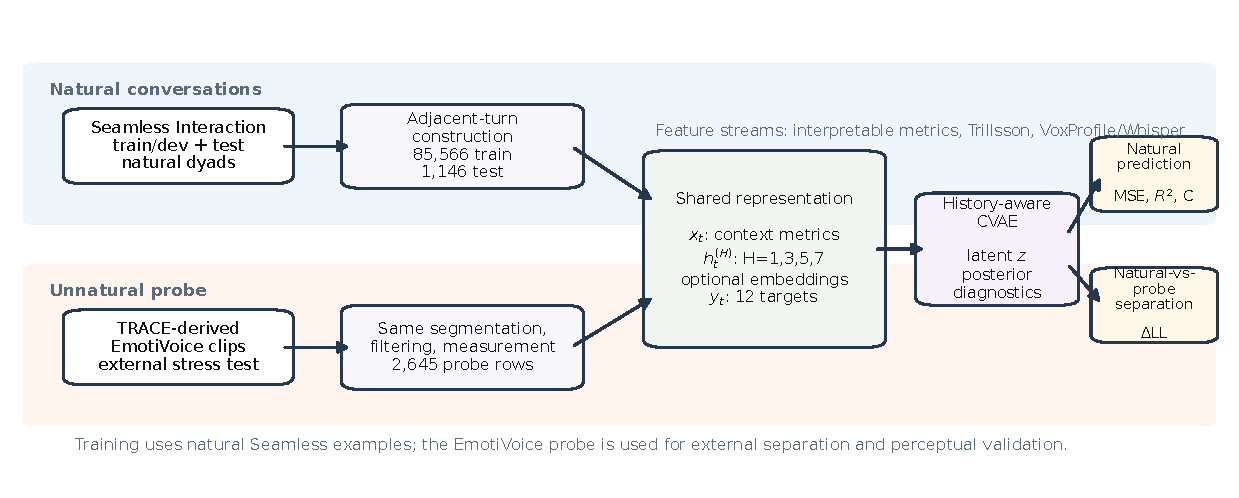
\includegraphics[width=0.95\textwidth]{figures/pipeline_schematic.pdf}
\caption{Evaluation pipeline. Natural Seamless conversations and TRACE-derived EmotiVoice probes are converted into adjacent-turn examples. Interpretable speech/context features and optional conditioning-turn embeddings feed a history-aware CVAE, whose outputs support natural-response prediction, natural-vs-unnatural likelihood gaps, and per-feature diagnostics.}
\label{fig:pipeline}
\end{figure*}

\section{Modeling and Evaluation}
\subsection{History-Aware CVAE}
The reported models are history-aware conditional variational autoencoders (CVAEs).
A transformer history encoder summarizes the padded history sequence using a learned CLS token, two transformer layers, four attention heads, hidden size 256, GELU activations, and a padding mask.
The current conditioning vector is projected separately and concatenated with the history summary.
The CVAE latent variable $z$ represents residual variability in response behavior that is not determined by the observed conversation context.
The encoder approximates $q_{\phi}(z \mid x_t,h_t^{(H)},y_t)$, and the decoder predicts a diagonal Gaussian distribution over $y_t$ from $(x_t,h_t^{(H)},z)$.
Training minimizes
\begin{equation}
    \mathcal{L} =
    -\log p_{\theta}(y_t \mid x_t,h_t^{(H)},z)
    + \beta D_{\mathrm{KL}}\left(q_{\phi}(z \mid x_t,h_t^{(H)},y_t) \parallel p(z)\right),
    \label{eq:cvae_loss}
\end{equation}
where $p(z)$ is a standard normal prior and the latent dimension is 16.

\subsection{Model Conditions}
We evaluate 16 conditions formed by crossing four history windows, $H\in\{1,3,5,7\}$, with four information settings.
The interpretable-only setting uses measured speech and context features without learned speech embeddings.
The Trillsson setting adds the Trillsson embedding stream.
The VoxProfile/Whisper setting adds the VoxProfile/Whisper stream.
The dual-embedding setting adds both streams.
All numeric features and embedding dimensions are scaled using training-set statistics.

\subsection{Evaluation Axes}
Natural-response prediction is evaluated on the held-out Seamless test set using target-averaged scaled MSE, target-averaged $R^2$, and C-index over the 12 response targets.
Unnaturalness separation is evaluated by applying the same preprocessing and model checkpoints to the TRACE-derived EmotiVoice examples and computing
\begin{equation}
    \Delta_{\mathrm{LL}} =
    \mathrm{LL}_{\mathrm{natural\ test}} -
    \mathrm{LL}_{\mathrm{EmotiVoice}},
\end{equation}
where larger values indicate lower model likelihood for the EmotiVoice probe than for held-out natural responses.
For the balanced score in Table~\ref{tab:clean_sweep}, we average two normalized ranks: the rank for natural-test MSE and the rank for $\Delta_{\mathrm{LL}}$.
This score is deliberately simple; it identifies conditions that are not extreme on only one axis.

The current likelihood values are posterior diagnostic scores, because the CVAE evaluation path uses $q_{\phi}(z \mid x_t,h_t^{(H)},y_t)$.
They should therefore be interpreted as held-out conditional fit and separation diagnostics, not as final deployable prior-predictive S2S scores.
A deployable evaluator should sample from $p(z)$ using only the conditioning turn and history, then compute predictive intervals and residuals for the candidate response.

\section{Results}
\subsection{Clean 12-Target Sweep}
Table~\ref{tab:clean_sweep} reports all aggregate results over the 12 naturalness targets in Table~\ref{tab:target_metrics}.
The best natural-response predictor is the interpretable-only model with five previous turns, with MSE 0.0250 and $R^2=0.9748$.
This indicates that direct measurements of the preceding turn and recent interaction history are highly informative for predicting natural response behavior.
However, the same model has a small natural-vs-EmotiVoice likelihood gap, showing that strong prediction of natural test examples is not the same as strong unnaturalness screening.

\begin{table*}[t]
\centering
\caption{Clean 12-target multiturn sweep. MSE, $R^2$, and C-index are averaged over the naturalness targets in Table~\ref{tab:target_metrics}. $\Delta$LL is natural-test likelihood minus TRACE-derived EmotiVoice likelihood; higher means stronger separation. Bold marks the best natural predictor, strongest discriminator, and top balanced tier.}
\label{tab:clean_sweep}
\scriptsize
\setlength{\tabcolsep}{2.8pt}
\begin{tabular}{lccccccc}
\toprule
Condition & $H$ & MSE & $R^2$ & C-index & Nat. LL & $\Delta$LL & Bal. score \\
\midrule
Interpretable only & 1 & 0.0332 & 0.9673 & 0.9758 & 0.127 & 0.205 & 0.433 \\
Interpretable only & 3 & 0.0339 & 0.9664 & 0.9756 & 0.237 & 0.306 & 0.367 \\
\textbf{Interpretable only} & \textbf{5} & \textbf{0.0250} & \textbf{0.9748} & 0.9750 & \textbf{0.967} & 0.115 & 0.533 \\
Interpretable only & 7 & 0.0297 & 0.9702 & 0.9755 & 0.790 & 0.153 & 0.433 \\
\midrule
\textbf{Trillsson} & \textbf{1} & 0.0284 & 0.9715 & \textbf{0.9810} & 0.407 & 1.263 & \textbf{0.800} \\
Trillsson & 3 & 0.0336 & 0.9675 & 0.9792 & -0.264 & 0.472 & 0.500 \\
Trillsson & 5 & 0.0400 & 0.9602 & 0.9782 & -1.235 & 0.092 & 0.067 \\
Trillsson & 7 & 0.0413 & 0.9615 & 0.9760 & -0.644 & 0.205 & 0.133 \\
\midrule
VoxProfile/Whisper & 1 & 0.0399 & 0.9632 & 0.9793 & -0.007 & 0.496 & 0.400 \\
\textbf{VoxProfile/Whisper} & \textbf{3} & 0.0275 & 0.9732 & 0.9800 & 0.523 & 1.096 & \textbf{0.800} \\
VoxProfile/Whisper & 5 & 0.0348 & 0.9683 & 0.9780 & 0.504 & 0.924 & 0.500 \\
\textbf{VoxProfile/Whisper} & \textbf{7} & 0.0414 & 0.9604 & 0.9785 & -0.811 & \textbf{1.556} & 0.500 \\
\midrule
Dual embedding & 1 & 0.0357 & 0.9654 & 0.9790 & -0.147 & 0.390 & 0.333 \\
Dual embedding & 3 & 0.0261 & 0.9738 & 0.9782 & 0.413 & 0.405 & 0.700 \\
Dual embedding & 5 & 0.0335 & 0.9672 & 0.9776 & 0.049 & 1.281 & 0.700 \\
\textbf{Dual embedding} & \textbf{7} & 0.0303 & 0.9706 & 0.9789 & -0.226 & 1.451 & \textbf{0.800} \\
\bottomrule
\end{tabular}
\end{table*}

\subsection{Prediction-Separation Tradeoff}
The strongest discriminator is VoxProfile/Whisper with $H=7$, which gives the largest likelihood gap ($\Delta$LL 1.556) but the weakest natural-test MSE among the 16 conditions.
Conversely, the best natural predictor, interpretable-only $H=5$, gives the smallest MSE but a much smaller likelihood gap.
The balanced score therefore identifies a top tier rather than a single universal winner: VoxProfile/Whisper $H=3$, Trillsson $H=1$, and dual embedding $H=7$ all receive score 0.800.
These three conditions occupy different parts of the tradeoff surface, as shown in Fig.~\ref{fig:tradeoff}.

\begin{figure*}[t]
\centering
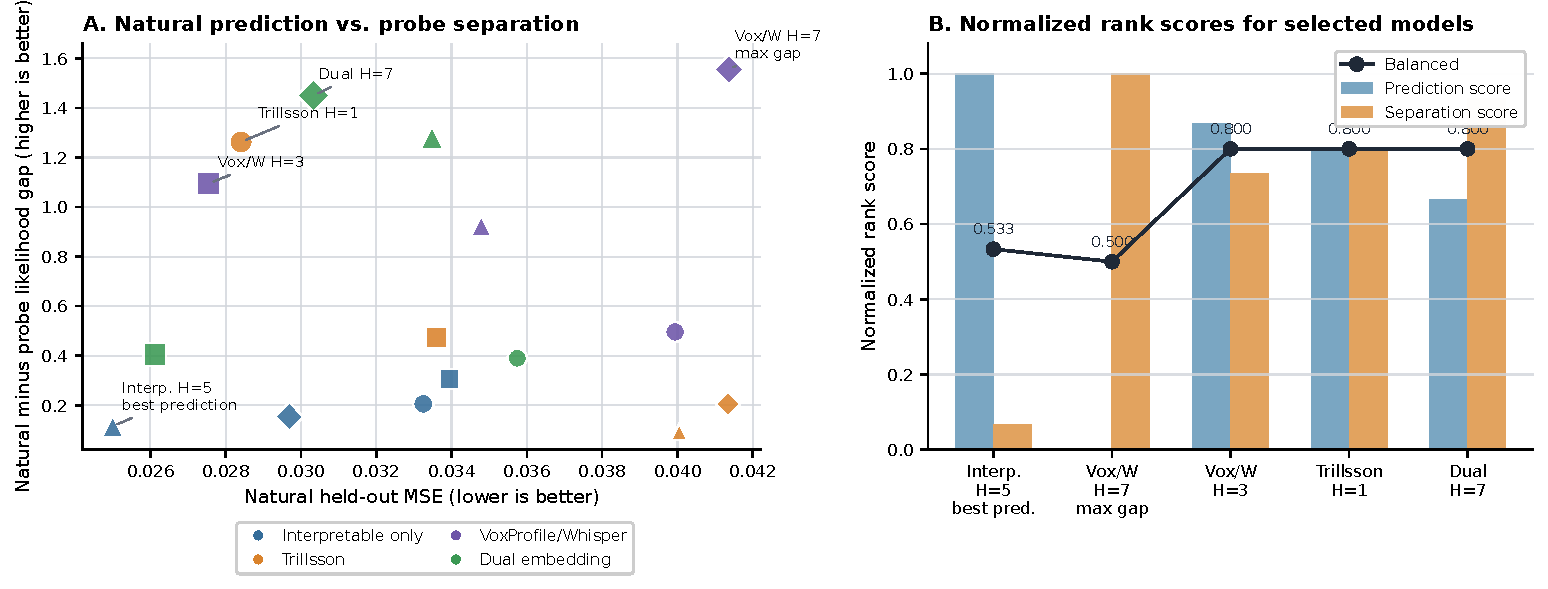
\includegraphics[width=0.95\textwidth]{figures/prediction_discrimination_scatter.pdf}
\caption{Prediction-separation tradeoff over the clean 12-target evaluation. The best natural predictor is the interpretable-only $H=5$ model, while the strongest EmotiVoice separator is VoxProfile/Whisper $H=7$. Marker size is proportional to the balanced score.}
\label{fig:tradeoff}
\end{figure*}

\subsection{Per-Feature Diagnostics}
Table~\ref{tab:per_feature} summarizes which model families are most useful for different target groups.
Interpretable features dominate prediction of duration, word count, rate, mean pause duration, arousal, and valence.
Embedding-augmented models are more useful for separation, especially for affect and pitch variation.
The largest per-feature likelihood gaps occur for arousal under Trillsson $H=1$ and dominance under dual embedding $H=7$, consistent with the intuition that the TRACE-derived EmotiVoice probe is most unnatural in affective and style-related dimensions.

\begin{table*}[t]
\centering
\caption{High-signal per-feature findings over the clean target space. Prediction winners use natural-test MSE; separation winners use per-feature $\Delta$LL.}
\label{tab:per_feature}
\scriptsize
\setlength{\tabcolsep}{3.2pt}
\begin{tabular}{p{0.16\textwidth}p{0.22\textwidth}p{0.23\textwidth}p{0.31\textwidth}}
\toprule
Target group & Strongest prediction & Strongest separation & Interpretation \\
\midrule
Duration and lexical length & Interpretable-only $H=1/7$ & VoxProfile/Whisper $H=5$; Trillsson $H=3$ & Turn length is well captured by measured context, while embeddings add signal for atypical response length. \\
Pitch and voicing & VoxProfile/Whisper $H=3$; dual embedding $H=3/7$ & VoxProfile/Whisper $H=7$ & Learned speech embeddings are useful for pitch-variation deviations. \\
Rate and pausing & Interpretable-only $H=5$; dual embedding $H=3$ & Trillsson $H=3/7$; interpretable-only $H=1$ & Segment-level rate and pausing depend on both recent context and acoustic style. \\
Affect & Interpretable-only $H=5$; dual embedding $H=3$ & Trillsson $H=1$; dual embedding $H=5/7$ & Arousal and dominance provide the clearest EmotiVoice separation. \\
\bottomrule
\end{tabular}
\end{table*}

\subsection{Human Perceptual Validation}
The automatic separation results are strengthened by TRACE's listening study over mixed two-speaker clips \cite{TRACE}.
The study contains 75 non-foil clips and 200 target ratings from 10 listeners, plus 20 foil ratings used for quality control.
Foils are excluded from Table~\ref{tab:human_eval}.
Listeners rated overall naturalness, speaking-style dimensions, emotion flow, and signal quality on 1--5 scales, and ratings are averaged at the clip level before condition summaries are computed.

\begin{table*}[t]
\centering
\caption{Human naturalness ratings for the TRACE perceptual validation set. Values are clip-level mean $\pm$ standard deviation on 1--5 scales, with foils excluded. Style avg. is the average of rhythm/timing, emphasis/stress, speed/rate, and pauses/phrasing. Natural/ref. combines Original and Original VC; EmotiVoice all combines EmotiVoice TTS and EmotiVoice TTS VC.}
\label{tab:human_eval}
\scriptsize
\setlength{\tabcolsep}{5.0pt}
\begin{tabular}{lccccc}
\toprule
Condition & $n$ & Overall & Style avg. & Emotion flow & Audio quality \\
\midrule
Original & 20 & $4.73 \pm 0.24$ & $4.75 \pm 0.29$ & $4.86 \pm 0.23$ & $4.80 \pm 0.38$ \\
Original VC & 20 & $4.25 \pm 0.51$ & $4.44 \pm 0.44$ & $4.33 \pm 0.58$ & $4.48 \pm 0.46$ \\
EmotiVoice TTS VC & 20 & $3.03 \pm 0.61$ & $3.33 \pm 0.77$ & $2.97 \pm 0.82$ & $4.22 \pm 0.53$ \\
EmotiVoice TTS & 15 & $2.32 \pm 0.77$ & $2.70 \pm 0.38$ & $2.39 \pm 0.76$ & $3.72 \pm 0.73$ \\
\midrule
Natural/ref. all & 40 & $4.49 \pm 0.47$ & $4.59 \pm 0.40$ & $4.60 \pm 0.51$ & $4.64 \pm 0.45$ \\
EmotiVoice all & 35 & $2.73 \pm 0.76$ & $3.06 \pm 0.70$ & $2.72 \pm 0.83$ & $4.01 \pm 0.66$ \\
\bottomrule
\end{tabular}
\end{table*}

Listeners rated natural/reference clips much higher than EmotiVoice clips in overall naturalness, 4.49 vs. 2.73 MOS, with a significant clip-level Mann--Whitney comparison ($p<0.001$).
The largest perceptual drops are in emotion flow, emphasis/stress, pauses/phrasing, and rhythm/timing.
Audio quality remains relatively high for EmotiVoice, especially after voice conversion, so the perceptual gap is not explained only by signal artifacts.
This study validates the EmotiVoice condition as an external unnaturalness probe; it does not yet establish per-item correlation between our likelihood scores and human adjacent-turn judgments.

\section{Discussion}
The results point to two complementary roles for the feature families.
First, the strongest natural-response predictor is not an embedding-heavy model; it is the interpretable-only $H=5$ condition.
This is encouraging because it means that directly measurable speech and context variables carry substantial information about natural response behavior.
Second, the models that best separate TRACE-derived EmotiVoice examples from held-out natural examples do use learned speech embeddings.
This suggests that embeddings capture acoustic or paralinguistic mismatch that is not fully represented by the 12 interpretable response targets.

These results support a two-axis view of S2S naturalness evaluation.
If the goal is to predict the range of natural response measurements, interpretable features with several turns of history are strongest.
If the goal is to screen for S2S/TTS-style unnaturalness, embedding-augmented models provide stronger separation.
The balanced top tier should be interpreted as a set of practical choices rather than a universal winner: VoxProfile/Whisper $H=3$ offers the best MSE among the balanced models, Trillsson $H=1$ offers a compact short-history option, and dual embedding $H=7$ offers strong separation at the cost of weaker prediction.

Several limitations remain.
The reported likelihoods are posterior CVAE diagnostics, not final prior-predictive S2S scores.
The TRACE-derived EmotiVoice probe is perceptually validated, but it represents one family of unnatural speech manipulations from a recent preprint, not the full space of S2S failure modes.
Finally, the listener study validates the external probe at the clip level; a future adjacent-turn listener study should correlate frozen prior-predictive scores and per-feature residuals with human judgments of response naturalness, conversational fit, timing, prosody, and signal quality.

\section{Conclusion}
We presented a conversation-context conditioned framework for evaluating S2S response naturalness through distributions over interpretable speech measurements.
The paper extends DISTRIB's reference-based prosody and rhythm checks from static matched regimes to learned conditional response distributions, and uses TRACE-derived EmotiVoice examples as an external unnaturalness probe.
Using a 12-metric naturalness target space, interpretable metric and context features with a five-turn history give the best held-out natural prediction, while embedding-augmented models provide stronger natural-vs-EmotiVoice separation.
Human ratings independently confirm that the EmotiVoice condition is perceived as less natural than natural/reference speech, especially in emotion flow and speaking style.
Future work will convert the posterior diagnostic into a prior-predictive evaluator and directly validate per-item scores against listener judgments.

\bibliographystyle{IEEEtran}
\bibliography{newbib}

\end{document}
